\subsection{Agile Softwareentwicklungsmodelle}
% \addcontentsline{toc}{subsection}{Agile Softwareentwicklungsmodelle}
\label{Agile Softwareentwicklungsmodelle}
Aufbauend auf den Ideen agiler Softwareentwicklung sind verschiedene agile Entwicklungsmodelle entstanden, von denen es einige zu großer Popularität gebracht haben. Das wohl bekannteste agile Softwareentwicklungsmodell ist \gls{SCRUM}.\newline
\gls{SCRUM} definiert ein Projekt als Abfolge iterativer Schritte, dem Produktbacklog. Der Backlog ist veränderbar. An bestimmten Stellen vor und nach einem Teilschritt (Sprint) können Veränderungen am Backlog vorgenommen werden. Dies umfasst z.B. das Hinzufügen oder Entfernen von Anforderungen oder die Re-Priorisierung bestehender Backlogelemente. Innerhalb des Gesamtprojektes werden Anforderungen in Sprints von begrenzter Dauer umgesetzt. Am Ende jeden Sprints steht ein lauffähiges Stück Software und Sprints verfügen über ihren eigenen Sprintbacklog. In diesem Backlog werden die Teilschritte der einzelnen Sprints gesammelt und priorisiert. Ein laufender Sprint kann nicht unterbrochen werden. Innerhalb eines Sprints wird die tägliche Arbeit zwischen den beteiligten Teammitgliedern über tägliche Meetings (Daily Scrum) synchronisiert, sodass auf Veränderungen und Verzögerungen direkt reagiert werden kann. Am Ende eines Sprints erfolgt ein Rückblick inklusive Bewertung, die s.g. Sprint Retrospektive. Die Erkenntnisse aus diesem Rückblick fließen in den nächsten Sprint mit, gleichzeitig werden die Items im Produktbacklog permanent aktualisiert und präzisiert. Die Zusammenhänge der Abläufe verdeutlicht die folgende Grafik in Anlehnung an \cite{SCRUM_Framework_nodate} und \cite[Abb. 1]{moniruzzaman2013comparative}:

\begin{center}
    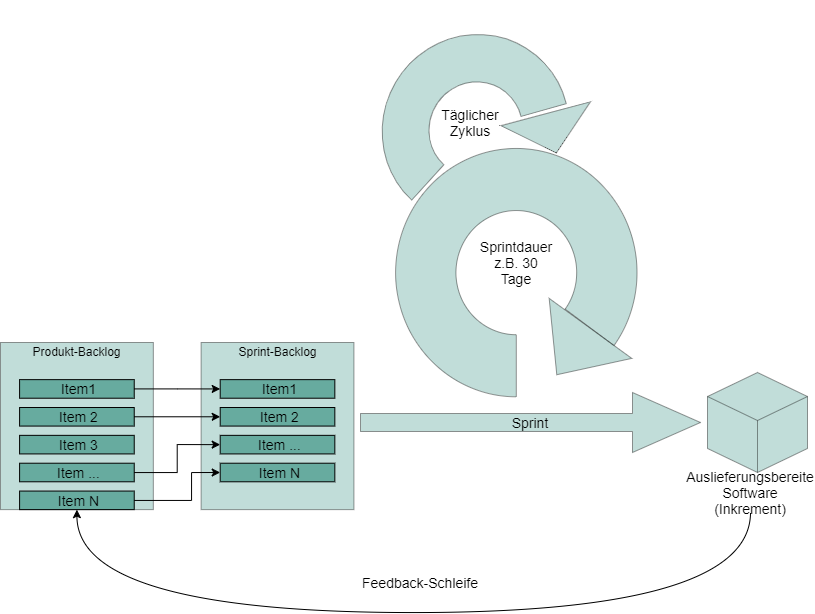
\includegraphics[width=0.8\textwidth]{Grafiken/SCRUM.png}
    \captionof{figure}{Ablauf des SCRUM-Modells}
    \label{Grafik:Ablauf des SCRUM-Modells}
\end{center}

Damit dieser vergleichsweise aufwändige Ablauf erfolgreich in der Praxis umgesetzt werden kann, setzt \gls{SCRUM} insbesondere auf zwischenmenschliche Kommunikation und Werte. Hierzu zählen insbesondere Offenheit, ein hohes Maß an Autonomie für die einzelnen Mitarbeiter, Transparent und Stringenz in den Abläufen \cite{SCRUM_values_nodate}.\newline
Ein weiterer prominenter Vertreter ist das in seinen Abläufen stark an das Spiralmodell angelehnte Extreme Programming (\acrshort{XP}). Erstmalig im Jahr 2000 von Kent Beck niedergeschrieben \cite{beck_extreme_2000}, etabliert \acrshort{XP} 13 Prinzipien, mit denen bewährte Methoden \glqq im Extremen\grqq{} betrieben, also im großen Maßstab eingesetzt werden sollen.
Diese Prinzipien umfassen Rollen der Projektbeteiligten vergleichbar mit denen des \gls{SCRUM}-Modells. Zudem gilt auch hier der Grundsatz aus Kundensicht zu denken, getane Arbeit iterativ zu integrieren (und dabei möglichst viel wiederzuverwenden). Softwaretests sind ein direkter Teil der Arbeitsschritte. Die nachfolgende Grafik verdeutlicht diese Zusammenhänge:

\begin{center}
    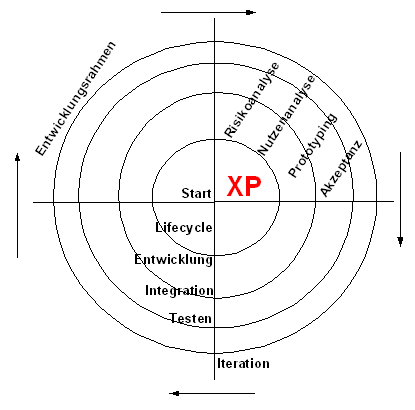
\includegraphics[width=0.6\textwidth]{Grafiken/XP-Life.png}
    \captionof{figure}{Zyklen des Extreme Programmings \cite{huttermann_xp_2006}}
    \label{Grafik:Zyklen des Extreme Programmings}
\end{center}

Zusammenfassend kann man festhalten, dass agile Softwareentwicklung und Softwareentwicklungsmodelle durch die folgenden Merkmale gekennzeichnet sind (in Anlehnung an \cite{moniruzzaman2013comparative} nach \cite{goos_extreme_2002}):
\begin{itemize}
    \item iterativ / wiederholend
    \item inkrementell / fortschreitend (das fertige Produkt wird nicht in einem Schritt erstellt)
    \item selbstorganisierend (insbesondere die Projektteams untereinander)
    \item aufstrebend (\glqq{}emergent\grqq{}), lernen also aus ihren eigenen Abläufen
\end{itemize}
Vor dem Hintergrund der vielen variablen Prozessbestandteile ist es wichtig zu beachten, dass agil ungleich beliebig ist.
Agile Softwareentwicklung kann erheblich einfacher auf wechselnde Anforderung reagieren als monolithische Modelle, trotzdem sind definierte Abläufe nicht änderbar. Änderungen sind nur an definierten Punkten möglich und agile Softwareentwicklung bedeutet daher nie unbegrenzte Flexibilität. 